% ******************************
%* FILE CONFIGURATION
% ******************************
\documentclass[12pt, a4paper]{article}

\usepackage[spanish, es-tabla]{babel} % Enables Spanish language support and table naming
\usepackage{hyperref} % Enables creation of hyperlinks in the document
\usepackage{graphicx} % Enables inclusion of images and figures
\usepackage{multirow} % Provides multirow functionality for tables
\usepackage{float} % Provides better control for floating elements like tables and figures
\usepackage[left=2.5cm, right=2.5cm, top=2cm, bottom=2cm]{geometry} % Sets page margins
\usepackage{fancyhdr} % Allows customization of headers and footers

\pagestyle{fancy}
\fancyhf{} % Clears all header and footer fields
\fancyfoot[C]{\thepage} % Centers the page number at the footer
\renewcommand{\headrulewidth}{0pt} % Removes the header line
\renewcommand{\footrulewidth}{0pt} % Removes the footer line

\fancypagestyle{plain} % Forces the same style on first page
{
  \fancyhf{}
  \fancyfoot[C]{\thepage}
  \renewcommand{\headrulewidth}{0pt}
  \renewcommand{\footrulewidth}{0pt}
}

\setlength{\arrayrulewidth}{0.5mm} % Adjusts table bstep width
\setlength{\tabcolsep}{5pt} % Adjusts spacing between table columns

\def\tablename{Tabla} % Changes the name of the table caption


% ******************************
%* NEW COMMANDS
% ******************************

% Creates a custom numbered step command (with bold numbers)
\newcounter{step}
\newcommand{\step}[1]
{
  \par\vspace{2ex}
  \stepcounter{step}
  \noindent\textbf{\arabic{step}.} #1\par\vspace{1ex}
}

% Creates a custon numbered step command (without bold numbers)
\newcounter{normalstep}
\newcommand{\normalstep}[1]
{
  \par\vspace{1ex}
  \stepcounter{normalstep}
  \noindent{\arabic{normalstep}.} #1\par\vspace{1ex}
}


% ******************************
%* PSEUDO-CARATULA
% ******************************

\title{TP 3: Redes de Difracción}
\author
{
  Caorsi Juan Ignacio, \href{jcaorsi@itba.edu.ar}{jcaorsi@itba.edu.ar} \\
  Dib Ian, \href{idib@itba.edu.ar}{idib@itba.edu.ar} \\
  Moschini Rita, \href{rmoschini@itba.edu.ar}{rmoschini@itba.edu.ar} \\
  Tamagnini Ana, \href{atamagnini@itba.edu.ar}{atamagnini@itba.edu.ar}
}

\date{Grupo 4 - 13/05/2025}

\begin{document}
\maketitle

% ******************************
%* SECCIONES DEL ARTICULO
% ******************************
COMENTARIOS ADIONALES ELIMINABLES:
\begin{itemize}
\item (rita) las figuras 1 y 2 deberian estar en método experimental pero como latex es latex las pone en resultados :/
\end{itemize}

\section{RESUMEN (ana)}
qué problema se abordó, de qué manera (es decir, con qué dispositivo experimental se trabajó) y cuáles fueron los principales resultados obtenido

\section{INTRODUCCIÓN (ian)}
conceptos teoricos
No es necesario realizar un desarrollo teórico exhaustivo
mencionar resultados teóricos q se van a poner
ecuaciones sobre magnitudes q seran medidas en la practica

\section{MÉTODO EXPERIMENTAL (rita)}
Se colocó de forma secuencial una lámpara de vapor de mercurio (la cual emitía un láser de $H_{e}N_{e}$), una lente convergente que enfocaba la imagen, la red de difracción a estudiar y una pantalla sobre la cual visualizar los máximos de interferencia de primer orden de las distintas longitudes de onda.

\subsection{Constante de la red}
Con la luz del láser se iluminó la red de difracción. Se pudieron observar a cada lado del máximo central varias líneas luminosas de color azul, verde, naranja y rojas na línea luminosa, indicando la ubicación del 1er máximo de interferencia (�� = 1; −1).
• Se mide la distancia 2Y entre ellos y la distancia D entre la pantalla y la red y se calculan sus
respectivas incertezas, D y Y.
• Sabiendo que la longitud de onda de la luz emitida por el láser es  = 632,8 nm, se obtiene la constante K de la red con la ecuación (2) con su correspondiente incerteza.

\begin{figure}[!h] 
        \centering 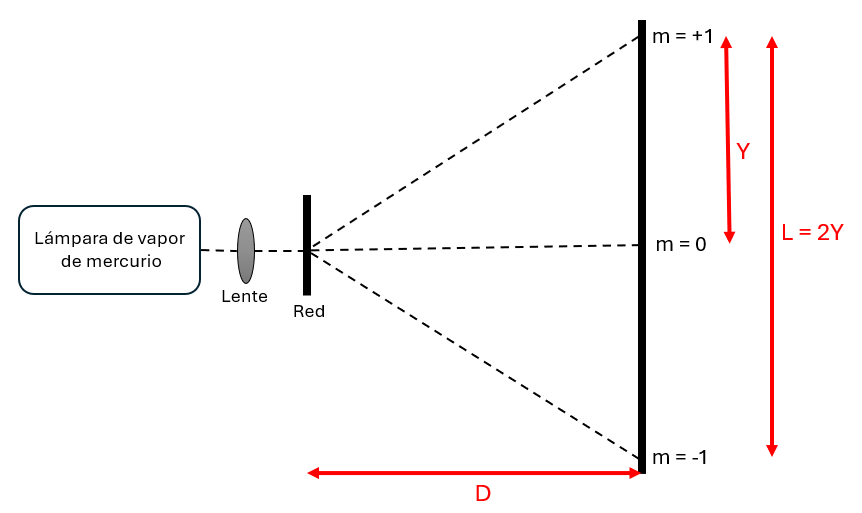
\includegraphics[width=0.5\columnwidth]{diagramaExperimental.png}
        \caption{\label{fig1}Diagrama de la disposición experimental, junto con las variables intervinientes.
        }
\end{figure}

\begin{figure}[!h] 
        \centering 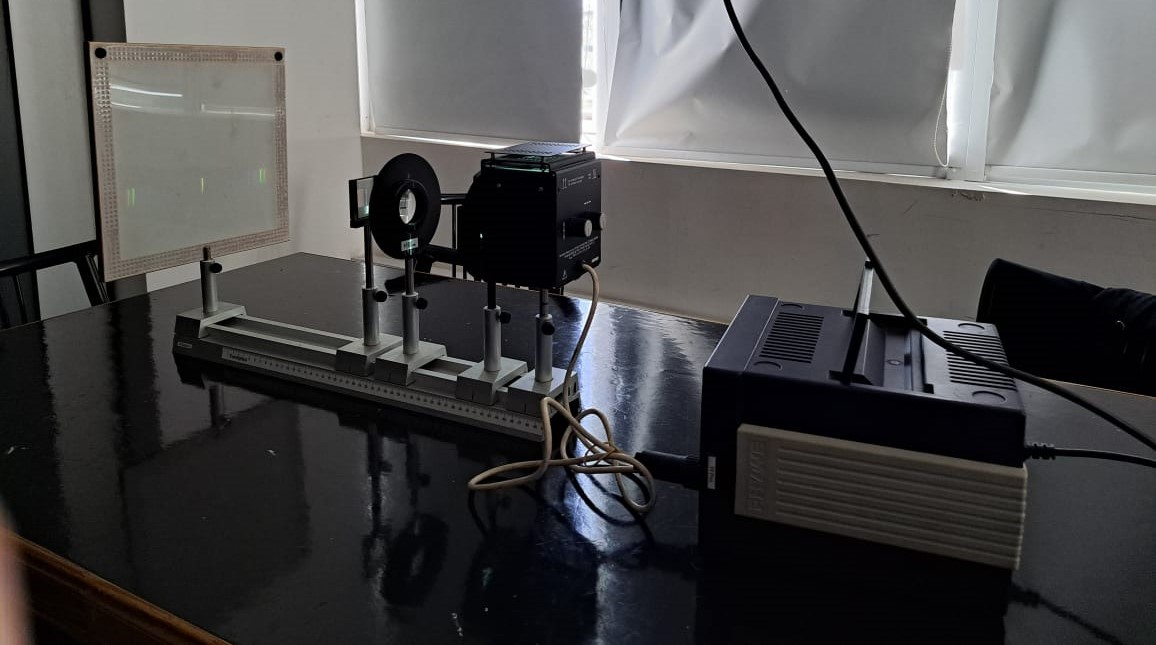
\includegraphics[width=0.5\columnwidth]{dispositivo2.jpg}
        \caption{\label{fig1}Foto de la disposición experimental en funcionamiento. De derecha a izquierda se pueden ver la fuente de alimentación, la lámpara de vapor de mercurio, la red de difracción, la lente y la pantalla.
        }
\end{figure}

\section{RESULTADOS (rita)}
resultados concretos
tablas, graficos
discusion de los resultados

\section{CONCLUSIONES (ian)}

\section{APÉNDICE: Cálculo de Incertezas}
%\addcontentsline{toc}{section}{Apéndice: Cálculo de Incertezas}
Entonces los valores buscados fueron los siguientes:

\subsection{Constante de la red}
busco K con los datos de la hoja de ian: y = 679 +- 10 mm, D = 1690 +- 1 mm.

\begin{equation}
  K = \frac{Y}{{\lambda} \sqrt{Y^{2} + D^{2}}}
\label{equation5}
\end{equation} 

y ${\Delta}K$ será:

\begin{equation}
  {\Delta}K = \sqrt{({\Delta}y)^2(\frac{D^{2}}{{\lambda} \left(Y^{2} + D^{2}\right)^{\frac{3}{2}}})^2+({\Delta}D)^2(-\frac{YD}{{\lambda} \left(D^{2} + Y^{2}\right)^{\frac{3}{2}}})^2}
\label{equation5}
\end{equation}

Obtengo K = 602.5 +-73.9 1/mm (para pasar a 1/cm que es lo que se pide en el informe lo podemos multiplicaar por 10).

\subsection{ Longitud de onda de las líneas azul, verde y roja de la luz emitida por la lámpara de mercurio.}
Sabemos que $D' = 296 +- 1 mm $ 
\begin{table}[H]
  \centering
  \begin{tabular}{|c|c|}
  \hline
  Color & Y \\
  \hline
  $Azul$  & 79 +- 1 mm  \\ \hline
  $Verde$  & 101.5 +- 1 mm \\ \hline
  $Amarillo$  & 107.5 +- 1 mm \\ \hline
  \end{tabular}
  \caption{\centering Valores de las longitudes entre máximos de las ondas (y, NO 2y)}
  \label{tabla1}
\end{table}

Para las longitudes de onda usamos:


\begin{equation}
  {\lambda} = \frac{Y}{K \sqrt{Y^{2} + D^{2}}}
\label{equation5}
\end{equation}

Con su incerteza:
\begin{equation}
  {\Delta}{\lambda} = \sqrt{({\Delta}K)^2(-\frac{Y}{\sqrt{Y^{2} + 
  D^{2}} \, K^{2}})^2 + ({\Delta}D)^2(-\frac{YD}{K \left(D^{2} + Y^{2}\right)^{\frac{3}{2}}})^2+ ({\Delta}Y)^2(\frac{D^{2}}{K \left(Y^{2} + D^{2}\right)^{\frac{3}{2}}})^2}
\label{equation5}
\end{equation}

Entonces los valores de las longitudes de onda son:
\begin{table}[H]
  \centering
  \begin{tabular}{|c|c|}
  \hline
  Onda por color & ${\lambda}$ \\
  \hline
  ${\lambda_{azul}}$  & 428.3 +- 52.7 nm  \\ \hline
  ${\lambda_{verde}}$  & 538.8 +- 66.2 nm \\ \hline
  ${\lambda_{amarillo}}$  & 567.0 +- 69.6 nm \\ \hline
  \end{tabular}
  \caption{\centering }
  \label{tabla2}
\end{table}


\end{document}
